\documentclass[10pt, a4paper]{beamer}
\usepackage{graphicx}
\graphicspath{{Demo_images/}}
\usetheme{Berkeley}
\usecolortheme{sidebartab}

\begin{document}
	\setbeamertemplate{sidebar left}{}
	\title{Progress Presentation-I}
	\subtitle{e-Yantra Summer Internship-2017 \\ Indoor Environments Mapping Using UAV}
	\author{Samaahita S Belavadi\\Rishabh Beri\\
	Mentors: Vamshi, Simranjeet}
	\institute{IIT Bombay}
	\date{\today}
	\frame{\titlepage}

\setbeamertemplate{sidebar left}[sidebar theme]
\section{Overview of Project}
\begin{frame}{Overview of Project}
	\begin{itemize}
		\item Project Name - Indoor Environments Mapping Using UAV
		\item Objective - The objective of this project is to map the indoor environments using a UAV equipped with a depth camera
		\item Deliverables -\\
		1) UAV with depth camera, processor mounted on it\\
		2) Code and Documentation for each task\\
		3) Video tutorials explaining solutions for each task
	\end{itemize}
\end{frame}

\section{Overview of Task}
\begin{frame}{Overview of Task}
\begin{tabular}{| c | p{6.5cm} | c | }
\hline
Task No. & ~~~~~~~~~~~~~~~~~~~~~~~~Task & Deadline\\
\hline
  1 & Install ROS, Control the quadrotor with keyboard in simulation & 25th May\\
\hline
2 & Land drone on an Aruco marker in simulation & 31st May\\
\hline
3 & Place Realsense R200 camera on the quadrotor model & 2nd June\\
\hline
4 & Generate 3D maps in simulation with keyboard controlled quadrotor & 6th June\\
\hline
5 & Literature review of autonomous mapping & 8th June\\
\hline
6 & Autonomously generate map in simulation & 17th June\\
\hline
7 & Interface Realsense with Cubieboard & 20th June\\
\hline
8 & Place setup of 3D camera and processor on drone & 22nd June\\
\hline
9 & Generate map in real time using drone (Manual control) & 27th June\\
\hline
10 & Project report & 3rd July\\
\hline
\end{tabular}
\end{frame}

\section{Task Accomplished}
\begin{frame}{Task Accomplished}
\begin{tabular}{| c | p{6.5cm} | c | }
\hline
Task No. & ~~~~~~~~~~~~~~~~~~~~~~~~Task & Status\\
\hline
  1 & Install ROS, Control the quadrotor with keyboard in simulation & Completed\\
\hline
2 & Land drone on an Aruco marker in simulation & Completed\\
\hline
3 & Place Realsense R200 camera on the quadrotor model & Completed\\
\hline
4 & Interface Realsense R200 camera with ROS on laptop and generate pointclouds & Completed\\
\hline
5 & Generate 3D maps in simulation with keyboard controlled quadrotor & Completed\\
\hline
\end{tabular}
\end{frame}

\section{Image - 1}
\begin{frame}{Image  - 1}
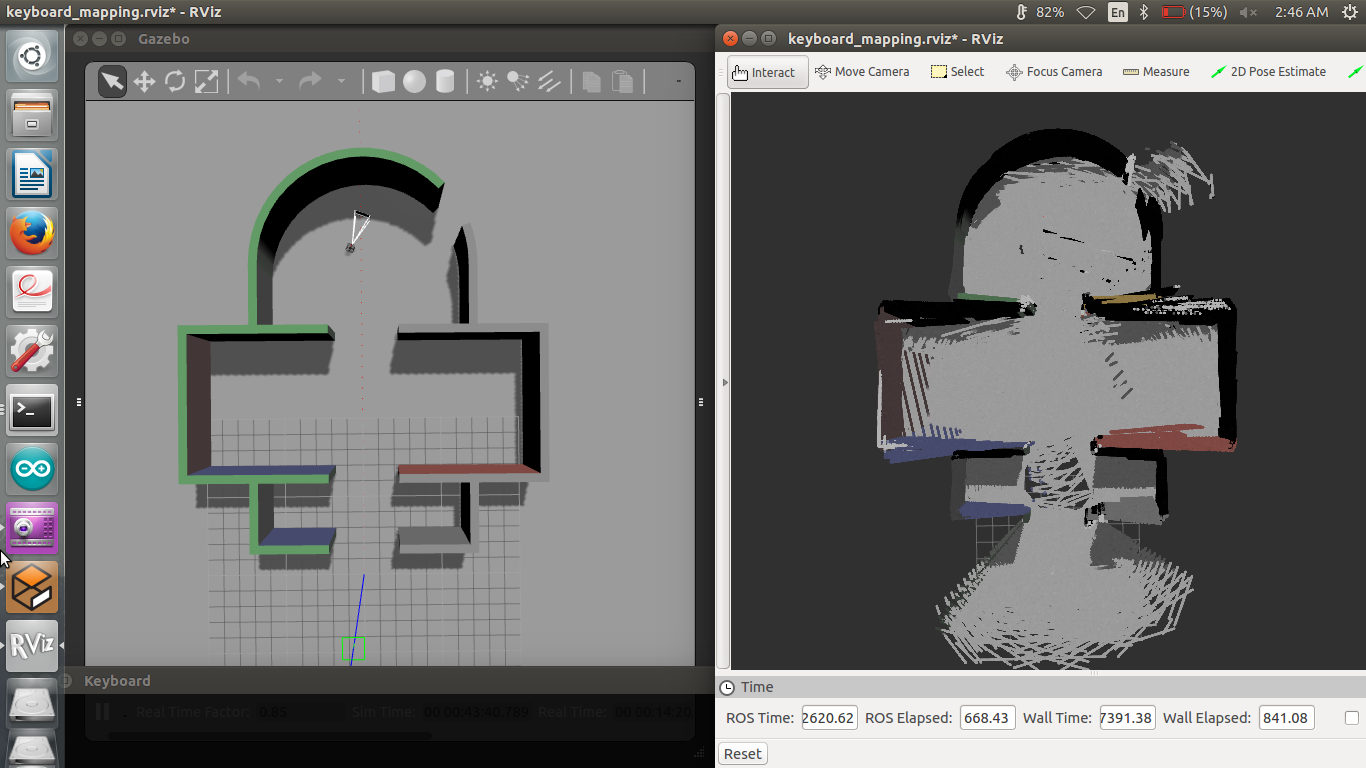
\includegraphics[scale = 0.2]{1.png}
\end{frame}

\section{Image - 2}
\begin{frame}{Image  - 2}
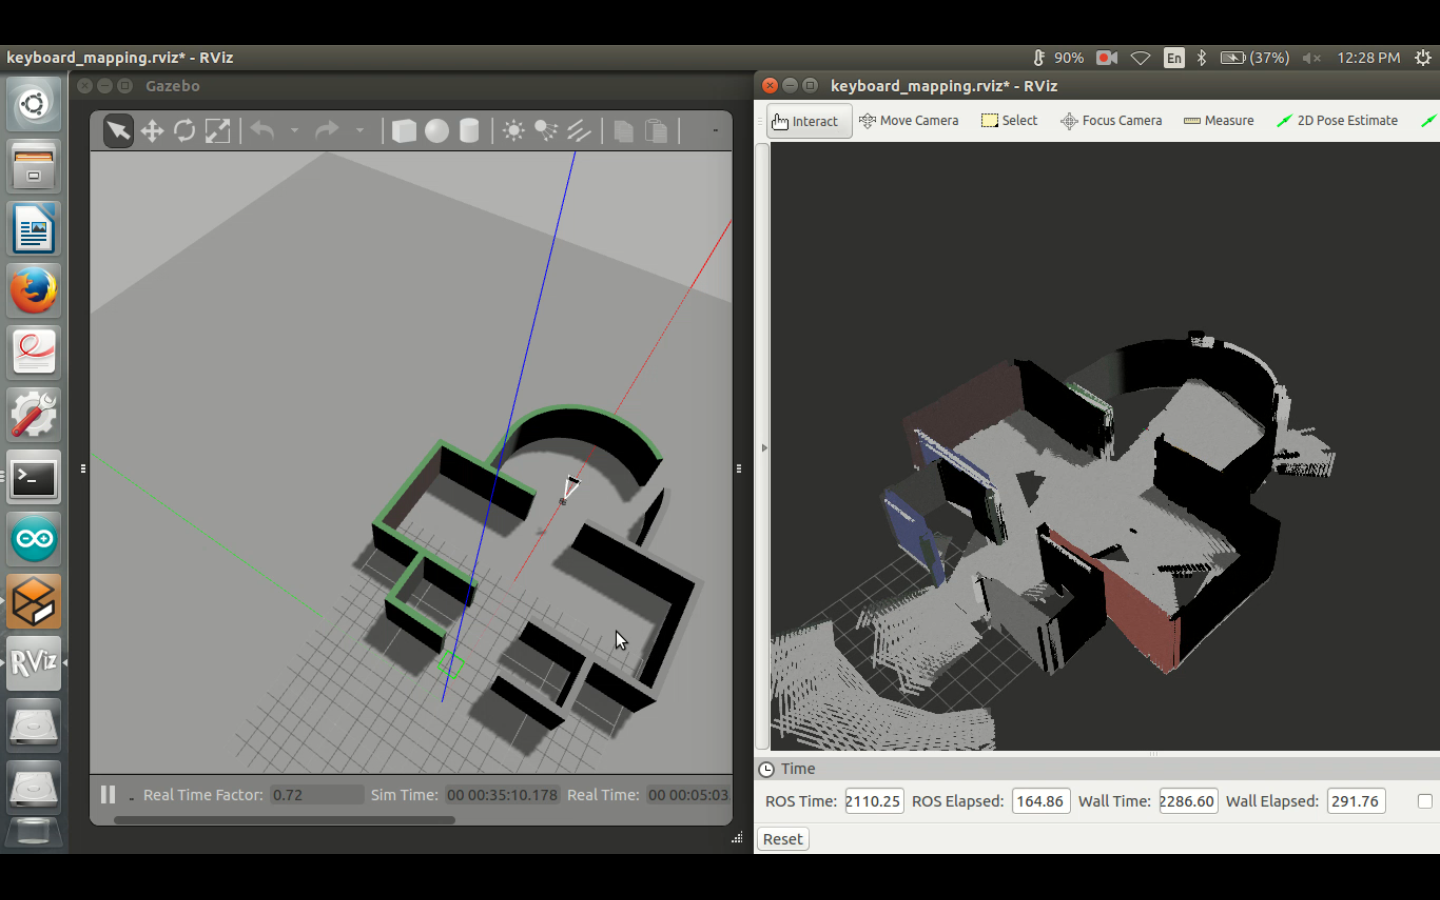
\includegraphics[scale = 0.2]{2.png}
\end{frame}

\section{Image -3}
\begin{frame}{Image - 3}
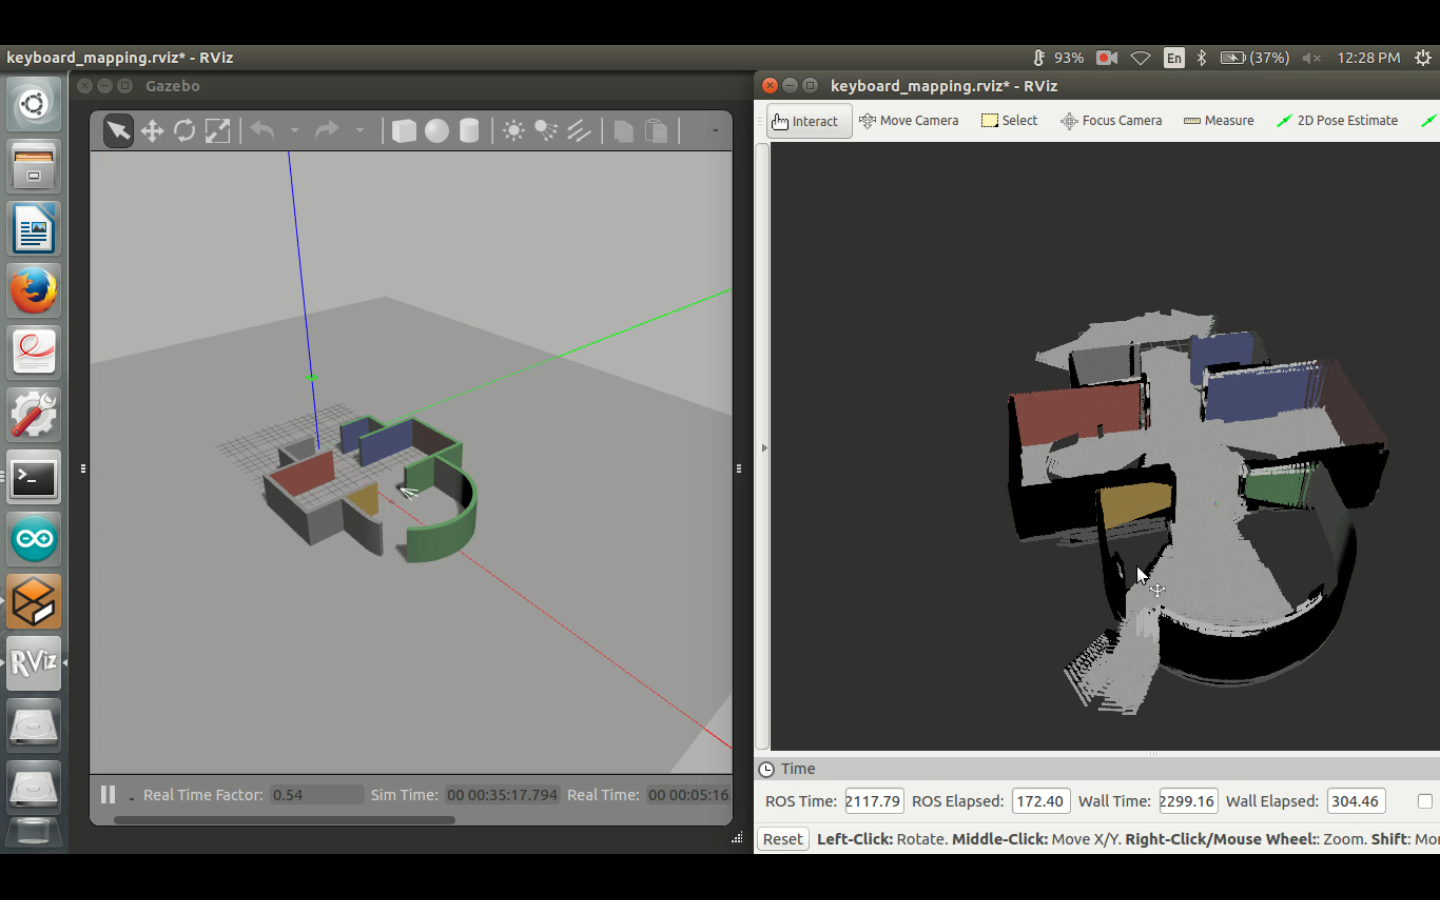
\includegraphics[scale = 0.2]{3.png}
\end{frame}

\section{Challenges Faced}
\begin{frame}{Challenges Faced}
	\begin{itemize}
		\item Tuning PID parameters for navigating the drone in simulation
		\item Realsense R200 camera model was in URDF format which is not supported by Gazebo
		\item The default encoding of the depth image is mono16 which had to be converted to 16UC1 for obtaining 3D point cloud data
		\item The frame of the depth image had to be changed to that of the color image for obtaining 3D point cloud data
	\end{itemize}
\end{frame}

\section{Future Plans}
\begin{frame}{Future Plans}
\begin{tabular}{| c | p{6.5cm} | c | }
\hline
Task No. & ~~~~~~~~~~~~~~~~~~~~~~~~Task & Deadline\\
\hline
1 & Literature review of autonomous mapping & 8th June\\
\hline
2 & Autonomously generate map in simulation & 17th June\\
\hline
3 & Interface Realsense with Cubieboard & 20th June\\
\hline
4 & Place setup of 3D camera and processor on drone & 22nd June\\
\hline
\end{tabular}
\end{frame}


\section{Thank You}
\begin{frame}{Thank You}
	\centering THANK YOU :)
\end{frame}
\end{document}
